\section{Experiments}
\subsection{Experimental Setups}
\subsubsection{Datasets}
We conduct experiments on six real-world tabular datasets: Adult~\cite{adult_2}, Anxiety~\cite{kaggleSocialAnxiety}, Compas~\cite{propublicaMachineBias}, Salary~\cite{kaggleGlobalMarket}, Obesity~\cite{obesity}, and Churn~\cite{churn}. These datasets cover a range of domains (e.g., social, medical, business) and downstream tasks including binary/multi-class classification and regression. Notably, Anxiety and Salary were released after the knowledge cutoff of modern LLMs, allowing us to assess performance in the absence of prior exposure. Full dataset details are provided in Appendix~\ref{app:datasets}. Additionally, for evaluating structure discovery quality, we utilize three benchmark datasets from bnlearn~\cite{scutari2010learning} with known ground-truth DAGs: Asia~\cite{bnlearn-repo-asia} (8 nodes), Child~\cite{bnlearn-repo-child} (20 nodes), and Insurance~\cite{bnlearn-repo-insurance} (27 nodes). These allow direct measurement of structural recovery via the Structural Hamming Distance (SHD)~\cite{de2009comparison}. 


\subsubsection{Baselines}
We compare our method against eleven baselines from three categories (implementation details in Appendix~\ref{app:baselines}): 1)~\textbf{Deep Generative Models (DGMs)}, including TVAE~\cite{xu2019modeling}, CTGAN~\cite{xu2019modeling}, TabDDPM~\cite{kotelnikov2023tabddpm}, NFlow~\cite{papamakarios2021normalizing}, and TabSyn~\cite{tabsyn}; 2)~\textbf{Structure-Aware Methods}, including Bayesian Networks~\cite{ankan2015pgmpy}, GOGGLE~\cite{liu2023goggle}, and DECAF~\cite{van2021decaf}; and 3)~\textbf{LLM-based Methods}, including GReaT~\cite{borisov2023language}, CLLM~\cite{cllm2024}, and GraDe~\cite{zhang-etal-2025-features}. 

\subsubsection{Evaluation Metrics}
We evaluate synthetic data quality along three axes (detailed definitions in Appendix~\ref{app:metrics}): \textbf{Downstream Model Performance} (AUC for classification, $R^2$ for regression, trained on $\mathcal{D}_{\mathtt{aug}} = \mathcal{D}_{\mathtt{train}} \cup \mathcal{D}_{\mathtt{synth}}$ and evaluated on $\mathcal{D}_{\mathtt{test}}$); \textbf{Statistical Fidelity} (mean pairwise correlation difference between real and synthetic data; \textbf{lower is better}); and \textbf{Privacy Risk}~\cite{van2023membership} (fraction of synthetic nearest neighbors from training set; \textbf{closer to 0.5 is better}).

\subsubsection{Implementation Details}

We use \texttt{gpt-4o-mini} with a temperature of 0.9 for both the CLLM and \textsf{StructSynth} models. Our experiments evaluate the low-data regime, generating 1000 synthetic samples ($s=1000$) from 100 original samples ($n=100$). Downstream performance is assessed using an XGBoost model. All experiments are repeated 10 times, and we report results as mean $\pm$ standard deviation to ensure robustness. Full hyperparameter configurations are provided in Appendix~\ref{app:hyperparameter}.


\begin{table*}[ht]
\centering
\caption{Comparison of Models on Privacy Preservation and Statistical Fidelity (\%). $^\dag$ indicates datasets created post LLM knowledge cutoff. Best results are in \textbf{bold}; second-best are \underline{underlined}.}

\resizebox{\textwidth}{!}{%
\small
\begin{tabular}{ll llllll cc}
\toprule

\textbf{Type} & \textbf{Method} & 
\multicolumn{1}{c}{\textbf{Adult}} &
\multicolumn{1}{c}{\textbf{Anxiety$^\dag$}} &
\multicolumn{1}{c}{\textbf{Compas}} &
\multicolumn{1}{c}{\textbf{Salary$^\dag$}} &
\multicolumn{1}{c}{\textbf{Obesity}} &
\multicolumn{1}{c}{\textbf{Churn}} &
\textbf{Average} & \textbf{Avg. Rank} \\

\midrule
\multicolumn{10}{l}{{Results for \textbf{Privacy Preservation}.} \textit{A value approaching 0.5 indicates better privacy preservation.}} \\
\midrule
    \multirow{5}{*}{DGMs} & TVAE & \underline{$50.34_{\pm 3.91}$} & $55.41_{\pm 4.26}$ & $64.50_{\pm 5.18}$ & $55.09_{\pm 4.38}$ & $52.93_{\pm 7.86}$ & $58.70_{\pm 4.75}$ & $56.16$ & $4.33$ \\
    & DDPM & $99.95_{\pm 0.05}$ & $66.20_{\pm 13.17}$ & $67.18_{\pm 18.06}$ & $63.32_{\pm 19.52}$ & $71.36_{\pm 16.88}$ & $62.89_{\pm 24.91}$ & $71.82$ & $9.67$ \\
    & CTGAN & $50.70_{\pm 3.64}$ & $56.64_{\pm 4.72}$ & $64.43_{\pm 4.22}$ & $53.59_{\pm 2.05}$ & $53.44_{\pm 3.89}$ & $57.84_{\pm 2.31}$ & $56.11$ & $4.67$ \\
    & NFlow & $54.36_{\pm 1.92}$ & $\boldsymbol{53.52_{\pm 3.08}}$ & \underline{$62.57_{\pm 3.66}$} & $52.76_{\pm 2.34}$ & $51.74_{\pm 3.68}$ & $52.97_{\pm 3.33}$ & $54.65$ & $3.50$ \\
    & TabSyn & $51.64_{\pm 2.67}$ & $70.53_{\pm 7.45}$ & $67.55_{\pm 5.40}$ & $54.66_{\pm 4.19}$ & $63.30_{\pm 7.19}$ & $59.38_{\pm 3.70}$ & $61.18$ & $7.50$ \\
\midrule
    \multirow{3}{*}{\makecell[l]{Structure\\Aware}} & GOGGLE & $49.15_{\pm 7.97}$ & $43.62_{\pm 33.49}$ & $65.16_{\pm 17.25}$ & $30.94_{\pm 18.49}$ & $44.28_{\pm 23.83}$ & $61.87_{\pm 18.01}$ & \underline{$49.17$} & $7.17$ \\
    & BN & $53.73_{\pm 2.36}$ & $72.98_{\pm 4.69}$ & $67.78_{\pm 3.63}$ & $61.50_{\pm 1.48}$ & $68.02_{\pm 2.18}$ & $59.68_{\pm 3.74}$ & $63.95$ & $8.83$ \\
    & DECAF & $46.23_{\pm 19.13}$ & $58.59_{\pm 10.37}$ & $64.07_{\pm 19.14}$ & $56.91_{\pm 17.41}$ & \underline{$50.82_{\pm 15.49}$} & $69.79_{\pm 18.81}$ & $57.74$ & $6.33$ \\
    \midrule
    \multirow{3}{*}{LLMs} & GReaT & $99.50_{\pm 0.35}$ & $85.39_{\pm 2.29}$ & $94.10_{\pm 1.33}$ & $86.66_{\pm 2.45}$ & $80.75_{\pm 2.99}$ & $94.51_{\pm 1.48}$ & $90.15$ & $11.83$ \\
    & CLLM & $49.45_{\pm 3.85}$ & $44.37_{\pm 4.55}$ & $64.14_{\pm 4.22}$ & \underline{$50.96_{\pm 5.40}$} & $45.36_{\pm 2.69}$ & $\boldsymbol{48.78_{\pm 5.82}}$ & $\boldsymbol{50.51}$ & \underline{$3.33$} \\
    & GraDe & $97.51_{\pm 1.60}$ & $61.14_{\pm 1.94}$ & $75.11_{\pm 5.11}$ & $65.99_{\pm 2.60}$ & $59.30_{\pm 4.76}$ & $69.07_{\pm 2.86}$ & $71.35$ & $9.50$ \\
    \midrule
    \multirow{1}{*}{Ours} & StructSynth & $\boldsymbol{49.97_{\pm 5.78}}$ & \underline{$44.74_{\pm 5.13}$} & $\boldsymbol{62.37_{\pm 3.86}}$ & $\boldsymbol{50.13_{\pm 4.89}}$ & $\boldsymbol{49.80_{\pm 6.31}}$ & \underline{$48.67_{\pm 4.84}$} & $50.95$ & $\boldsymbol{1.33}$ \\

\midrule
\midrule
\multicolumn{10}{l}{{Results for \textbf{Statistical Fidelity}.} \textit{A lower score indicates higher fidelity.}} \\
\midrule
    \multirow{5}{*}{DGMs} & TVAE & $53.71_{\pm 1.80}$ & $46.16_{\pm 1.28}$ & $60.26_{\pm 1.09}$ & $66.93_{\pm 1.13}$ & \underline{$58.41_{\pm 0.52}$} & $53.22_{\pm 1.54}$ & $58.11$ & $5.17$ \\
    & DDPM & $65.26_{\pm 1.05}$ & $52.76_{\pm 1.22}$ & $64.94_{\pm 1.79}$ & $90.51_{\pm 0.33}$ & $64.44_{\pm 1.36}$ & $64.40_{\pm 2.90}$ & $67.05$ & $10.00$ \\
    & CTGAN & \underline{$52.37_{\pm 1.56}$} & $47.14_{\pm 2.39}$ & $59.96_{\pm 0.90}$ & $58.57_{\pm 0.89}$ & $58.71_{\pm 0.57}$ & \underline{$52.32_{\pm 1.75}$} & $54.85$ & \underline{$4.17$} \\
    & NFlow & $\boldsymbol{50.68_{\pm 2.71}}$ & \underline{$43.50_{\pm 1.77}$} & $60.62_{\pm 0.93}$ & \underline{$52.38_{\pm 1.10}$} & $58.85_{\pm 0.98}$ & $53.98_{\pm 2.24}$ & $\boldsymbol{53.34}$ & $4.50$ \\
    & TabSyn & $49.17_{\pm 1.34}$ & $55.31_{\pm 1.31}$ & $57.23_{\pm 2.24}$ & $62.90_{\pm 3.01}$ & $58.08_{\pm 0.54}$ & $53.99_{\pm 2.08}$ & $56.11$ & $4.75$ \\
\midrule
    \multirow{3}{*}{\makecell[l]{Structure\\Aware}} & GOGGLE & $68.32_{\pm 1.38}$ & $51.58_{\pm 7.27}$ & $66.19_{\pm 1.13}$ & $87.15_{\pm 1.65}$ & $63.80_{\pm 2.40}$ & $65.51_{\pm 2.16}$ & $67.09$ & $10.00$ \\
    & BN & $82.68_{\pm 1.35}$ & $82.77_{\pm 2.39}$ & $60.13_{\pm 3.46}$ & $\boldsymbol{46.33_{\pm 7.29}}$ & $59.76_{\pm 3.46}$ & $88.85_{\pm 3.02}$ & $70.09$ & $8.17$ \\
    & DECAF & $62.71_{\pm 3.21}$ & $48.53_{\pm 1.53}$ & $63.82_{\pm 1.34}$ & $84.70_{\pm 2.41}$ & $60.93_{\pm 2.21}$ & $60.22_{\pm 0.88}$ & $63.49$ & $8.17$ \\
    \midrule
    \multirow{3}{*}{LLMs} & GReaT & $82.71_{\pm 1.35}$ & $\boldsymbol{40.10_{\pm 1.64}}$ & $\boldsymbol{52.17_{\pm 1.18}}$ & $58.75_{\pm 0.89}$ & $\boldsymbol{56.83_{\pm 0.87}}$ & $\boldsymbol{48.18_{\pm 2.16}}$ & \underline{$56.46$} & $\boldsymbol{3.33}$ \\
    & CLLM & $61.93_{\pm 4.43}$ & $57.64_{\pm 1.51}$ & $59.74_{\pm 2.33}$ & $78.60_{\pm 0.98}$ & $65.74_{\pm 1.42}$ & $62.20_{\pm 3.68}$ & $64.31$ & $8.50$ \\
    & GraDe & $84.30_{\pm 0.86}$ & $42.59_{\pm 0.93}$ & $53.82_{\pm 2.62}$ & $55.85_{\pm 1.42}$ & $57.44_{\pm 1.43}$ & $53.66_{\pm 1.90}$ & $57.94$ & \underline{$4.17$} \\
    \midrule
    Ours & StructSynth & $57.60_{\pm 3.13}$ & $57.86_{\pm 1.98}$ & \underline{$57.23_{\pm 1.69}$} & $64.64_{\pm 0.96}$ & $61.14_{\pm 1.10}$ & $58.63_{\pm 2.66}$ & $59.52$ & $7.08$ \\
\bottomrule
\end{tabular}}%
\label{tab:results_comparison_merged}

\end{table*}

\subsection{Main Results}
\subsubsection{Downstream Model Performance}
Table~\ref{tab:results_comparison_performance} summarizes the downstream results. \textsf{StructSynth} achieves the best mean performance on all six datasets, with a perfect average rank of 1.00 and the highest average score (75.01). This improves over using only $\mathcal{D}_\mathtt{train}$ (71.54) and surpasses CLLM (73.36), demonstrating that explicitly guiding an LLM with a structural blueprint yields substantial gains. Standard DGMs and structure-aware models perform notably weaker, as implicit learning and data-driven graph discovery are unreliable when training samples are scarce.



\subsubsection{Privacy Preservation and Statistical Fidelity}

Table~\ref{tab:results_comparison_merged} reveals a fundamental tension between fidelity and privacy. High statistical fidelity often stems from memorization: for example, GReaT achieves the best fidelity (avg.\ rank 3.33) but exhibits severe privacy risk (90.15\%), essentially reproducing training records. \textsf{StructSynth} achieves the best privacy preservation (avg.\ rank 1.33), outperforming CLLM (avg.\ rank 3.33), while maintaining competitive statistical fidelity (avg.\ rank 7.08). We attribute this to the explicit structural blueprint acting as a regularizer: it constrains overfitting to individual records while preserving the dependency structure that drives downstream utility.


\begin{figure*}[t!]
\centering
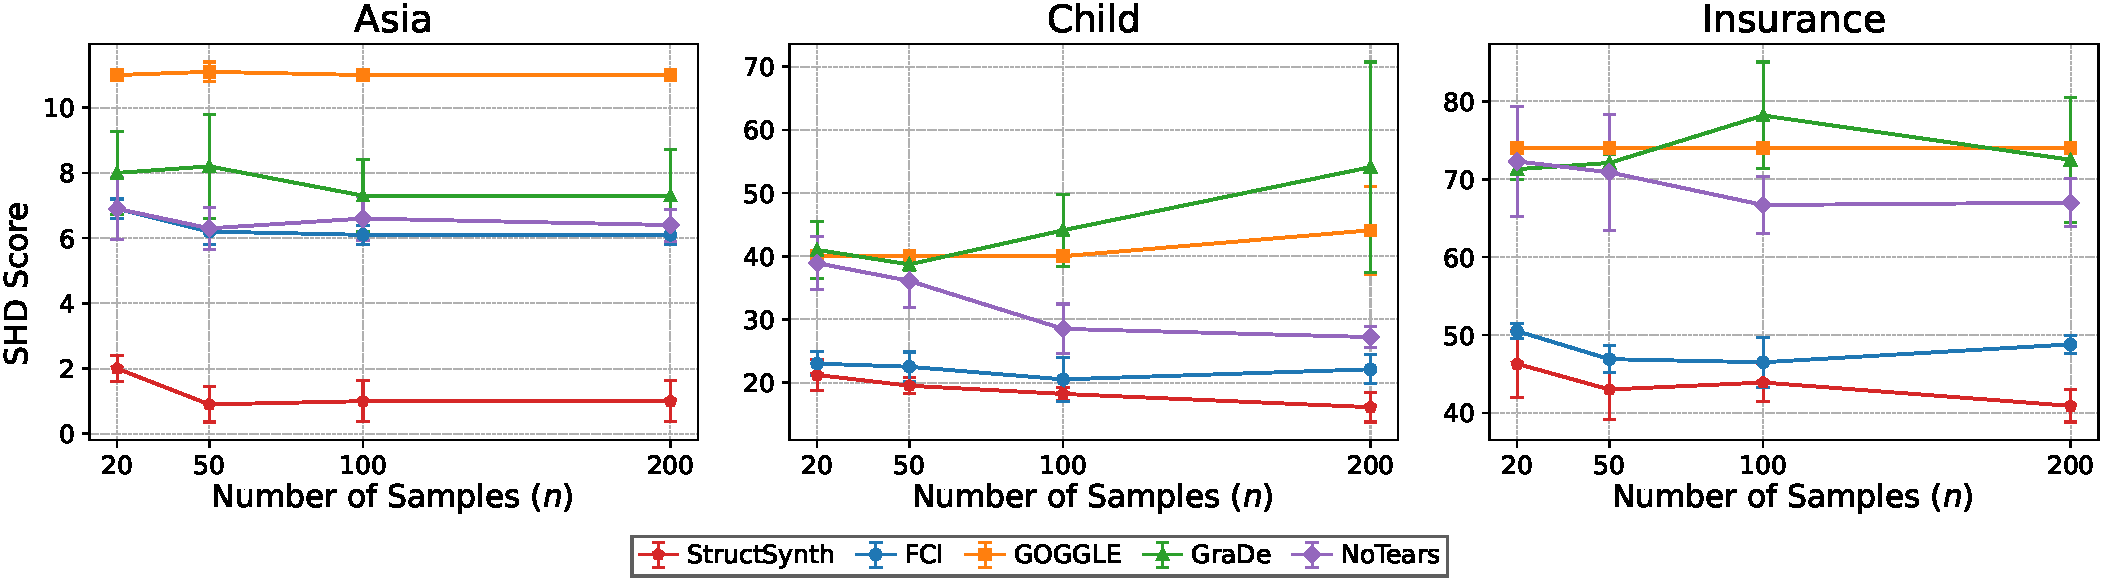
\includegraphics[width=\textwidth]{figures/shd_comparison_acm.pdf}
\caption{SHD of discovered dependency graphs vs. number of training samples on Asia, Child, and Insurance datasets with ground-truth DAGs. Lower SHD indicates better structural recovery.}
\label{fig:shd}
\end{figure*}




\subsection{Ablation Study}

To isolate the contributions of our method's two main stages, we evaluate seven variants. For the structure learning stage: 1) \textit{PC Discovery}, substituting our LLM-guided discovery with the classical Peter--Clark algorithm~\cite{spirtes2000causation}; 2) \textit{NoTears Discovery}, replacing our method with the continuous optimization-based NoTears algorithm~\cite{zheng2018dags}; 3) \textit{No-Correlation Score}, removing statistical correlation scores from the prompt to examine their guiding influence; and 4) \textit{Pairwise Discovery}, replacing the efficient BFS traversal with less scalable pairwise queries to evaluate the performance-efficiency trade-off. For the data generation stage: 5) \textit{No Topological Order}, conducting data generation based on the complete learned structure but ignoring the topological order; 6) \textit{No Structure}, removing structural guidance entirely (equivalent to the CLLM); and 7) \textit{Bayesian Sampler}, substituting the LLM generator with a traditional Bayesian sampler fitted to the learned graph.



\begin{table}[t!]
\small
\centering

\caption{Ablation Study on Adult Datasets.}
\setlength{\tabcolsep}{1mm}
\begin{tabular}{ll|ccc}
    \hline
    \multicolumn{2}{c|}{\textbf{Method}} & \textbf{AUC} & \textbf{Fidelity} & \textbf{Privacy} \\ 
    \hline
    \multicolumn{2}{c|}{\textsf{StructSynth}}& \textbf{85.55} & 57.96 & \underline{49.97} \\
    \hline
    \multirow{4}{*}{\makecell[l]{Structure\\Learning}} & PC Discovery& 84.54 & 59.69 & 50.52 \\
    & NoTears Discovery& 84.17 & 59.49 & 47.85 \\
    & No-Correlation Score& 84.06 & 59.10 & 46.60 \\
    & Pairwise Discovery & \underline{85.25} & 57.37 & 49.17 \\
    \hline
    \multirow{3}{*}{Generation} & No Topological Order & 84.41 & 60.47 & 51.03 \\
    & No Structure & 83.95 & 60.67 & 49.45 \\
    & Bayesian Sampler & 81.17 & \textbf{48.86} & \textbf{50.02} \\
    \hline
\end{tabular}

\label{tab:ablation_study}

\end{table}

The results, summarized in Table \ref{tab:ablation_study}, offer three key insights. First, \textbf{LLM-guided discovery outweighs classical baselines}: \textsf{StructSynth} outperforms both \textit{PC} and \textit{NoTears} (by 1.0--1.4 AUC pts). This suggests that leveraging semantic priors helps identify robust structures in low-data regimes where pure statistical methods often fail. Second, \textbf{structural guidance is multifaceted}: removing the graph (\textit{No Structure}) or ignoring its hierarchy (\textit{No Topological Order}) both degrade utility (by 1.6 and 1.1 pts), proving that both explicit dependencies and their correct causal ordering are essential. Finally, \textbf{synergy is vital}: replacing the LLM with a \textit{Bayesian Sampler} causes the sharpest drop (--4.4 pts), confirming that structural blueprints effectively guide---but cannot replace---the LLM's superior distributional learning capabilities. Additionally, removing statistical prompts (\textit{No-Correlation}) degrades performance, highlighting their value as weak supervision.


% The results, summarized in Table \ref{tab:ablation_study}, confirm that the framework's success stems from the synergy between the discovered graph and the LLM's generative power. Our central finding is that graph awareness is critical. Removing the structural guidance (\textit{No Structure}) significantly reduces AUC by 1.6 pts. More dramatically, replacing the LLM with a Bayesian Sampler yields the largest performance drop (–4.4 pts). This confirms the vital synergy between the learned graph and the LLM's generative capabilities—neither component is sufficient in isolation. We also find that prompt signals matter, as using \textit{No-Correlation} degrades AUC by 1.5 pts, highlighting their utility as a form of weak supervision.



\subsection{Structural Fidelity under Ground-Truth Graphs}

To rigorously evaluate the quality of the discovered structures, we employ three benchmark datasets from the \texttt{bnlearn} repository---Asia, Child, and Insurance---which possess known ground-truth DAGs. This allows us to directly quantify structural fidelity using the Structural Hamming Distance (SHD), which is standard in the literature and measures the number of edge insertions, deletions, or reversals required to transform the learned graph into the ground truth. A lower SHD indicates a more accurate recovery of the underlying causal mechanisms.

Figure \ref{fig:shd} presents the SHD across varying training sample sizes ($n \in \{20, 50, 100, 200\}$). \textsf{StructSynth} consistently achieves the lowest or near-lowest SHD across all datasets, demonstrating superior stability in low-data regimes. In contrast, traditional constraint-based methods like FCI and score-based methods like GOGGLE often yield significantly higher errors, particularly when $n$ is small.

On the \textbf{Asia} dataset, which is small but prone to spurious correlations in low-sample settings, \textsf{StructSynth} maintains an SHD near 1, whereas baselines fluctuate at much higher error rates. This suggests that our LLM-guided approach effectively utilizes prior knowledge to filter out false positives that purely statistical methods might mistake for true edges. For the \textbf{Child} dataset, which features a more complex structure, errors in early discovery stages can cascade. \textsf{StructSynth}'s iterative cycle resolution helps maintain graph validity, preventing the explosion of erroneous edges seen in methods like GraDe. Finally, on the \textbf{Insurance} dataset, which represents a medium-scale network with denser connections, our method again outperforms competitors. By prioritizing the discovery of a stable "structural blueprint" rather than attempting to model every minor correlation, \textsf{StructSynth} avoids the overfitting pitfalls that lead to the dense, incorrect graphs produced by some deep generative baselines. These results validate the first stage of our framework: \textsf{StructSynth} reliably identifies a high-fidelity dependency structure even from limited data, which is crucial for ensuring the subsequent generation follows valid causal pathways. We provide detailed examples on the 
Asia dataset in Appendix~\ref{app:qualitative_graph_analysis}.


\subsection{Influence of Training Sample Size}

\begin{figure*}[t!]
\centering
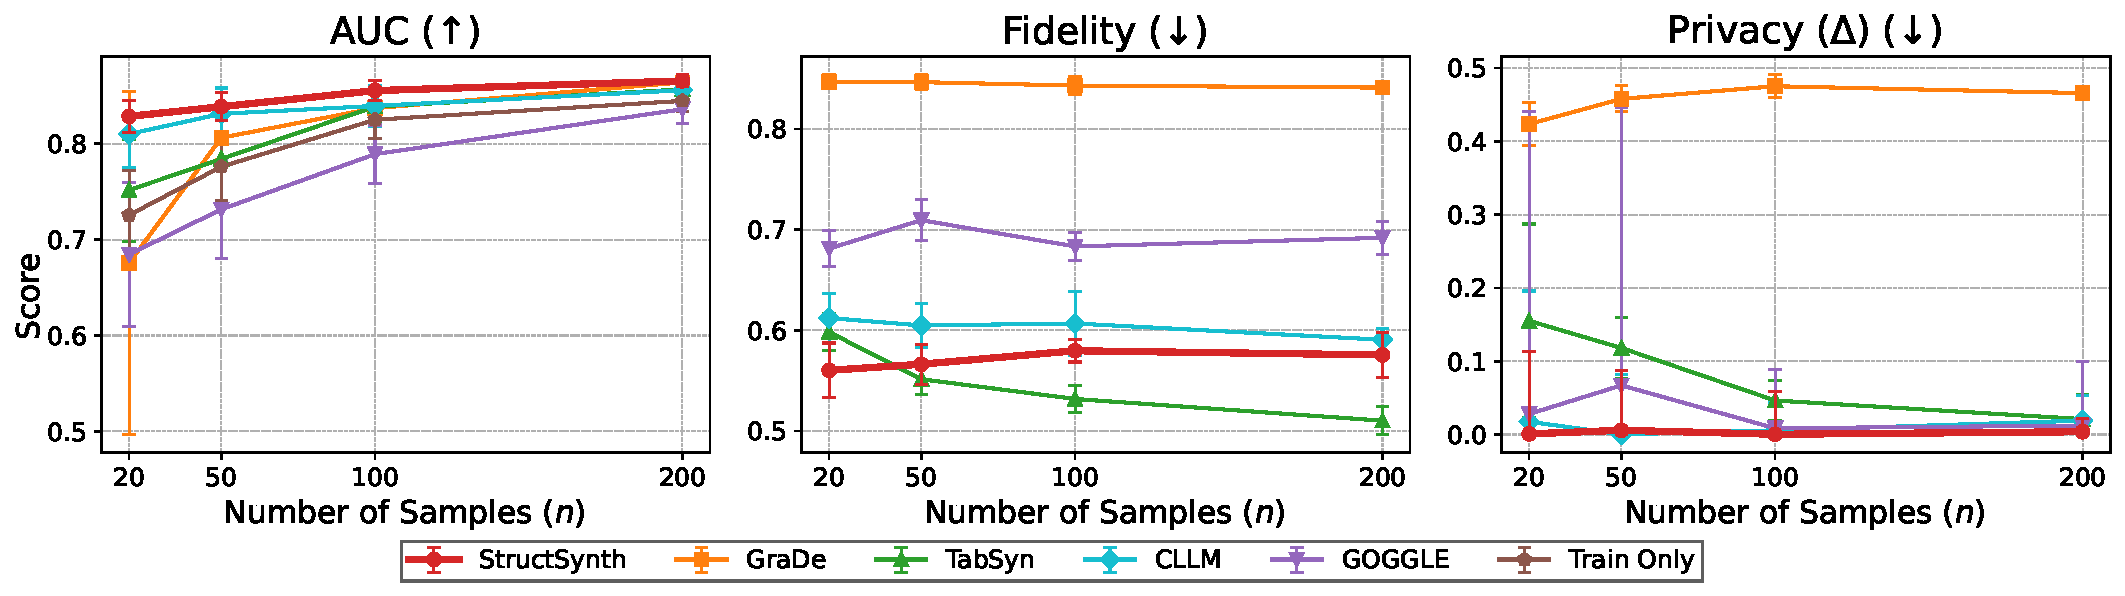
\includegraphics[width=\textwidth]{figures/influence_n/vary_n_all.pdf}
\caption{Effect of training sample size ($n$) on downstream utility (AUC$\uparrow$), statistical fidelity ($\downarrow$), and privacy risk deviation $\Delta$ ($\downarrow$) on the Adult dataset.}
\label{fig:influence_n}
\end{figure*}

\begin{figure}[h]
\centering
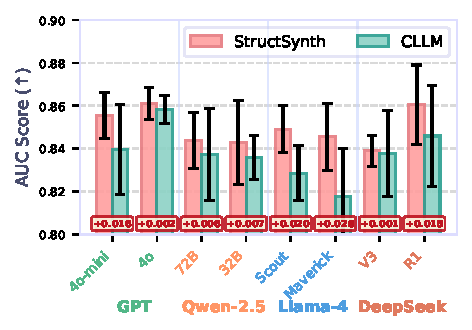
\includegraphics[width=\columnwidth]{figures/llm_compare.pdf}
\caption{AUC Score on the Adult Dataset Using Various LLMs for \textsf{StructSynth} and CLLM.}
\label{fig:llm_compare}
\end{figure}


To evaluate data efficiency, we varied the training size $n$ from 20 to 200 on the Adult dataset and measured AUC, Statistical Fidelity, and Privacy Risk deviation $\Delta$ (Figure \ref{fig:influence_n}). Regarding AUC, \textsf{StructSynth} consistently outperforms all baselines. Notably, in the low-data regime ($n\leq 50$), it maintains a high baseline, whereas methods like BN and GOGGLE require significantly more samples to become competitive.

For Statistical Fidelity, \textsf{StructSynth} maintains a stable low score across all sample sizes. In contrast, baselines often fail to improve fidelity synchronously with AUC, drifting towards erroneous correlations. This confirms that our explicit structural blueprint aligns the generated distribution with real dependencies early on, minimizing statistical distortion even with limited data. Regarding privacy, we report the deviation $\Delta = |\text{PrivacyRisk} - 0.5|$. \textsf{StructSynth}'s $\Delta$ remains negligible across all $n$, indicating no tendency towards memorization. Conversely, baselines often exhibit larger $\Delta$, reflecting the privacy-fidelity tension noted in Table \ref{tab:results_comparison_merged}. Our decoupled structure acts as a regularizer, preventing record-level overfitting. Overall, \textsf{StructSynth} exhibits a robust Pareto-like behavior: from low- ($n=20$) to mid-data ($n=200$) regimes, it simultaneously achieves high AUC, low Fidelity scores, and minimal Privacy $\Delta$, offering a stable trade-off independent of sample size.



\subsection{Influence of Different Language Models}

To assess the generalizability of \textsf{StructSynth}, we benchmark its performance against the CLLM baseline using a diverse set of LLMs on the Adult dataset. The evaluation spans a range of model sizes and includes both leading open-source models (Qwen-2.5~\cite{team2024qwen2}, Llama-4~\cite{meta2025llama4}, and DeepSeek~\cite{liu2024deepseek, guo2025deepseek} series) and proprietary models (GPT-4o~\cite{hurst2024gpt} series), thereby highlighting the versatility of our approach. Experimental settings are kept consistent with those described in the main experiments, with the exception that, due to the high inference cost of DeepSeek R1, its evaluation is limited to 100 synthetic samples (i.e., $s=100$).

The results, presented in Figure \ref{fig:llm_compare}, reveal a consistent and robust performance advantage for \textsf{StructSynth}. Our method outperforms the CLLM across every tested architecture, from open-source models of varying sizes to powerful proprietary ones. Interestingly, the magnitude of this performance gain is most significant for models like Maverick (+0.028 AUC), demonstrating that our structural guidance can substantially boost the performance of models with moderate native capabilities. Even for top-tier models like GPT-4o, which are highly capable on their own, \textsf{StructSynth} still provides a measurable improvement. This overall pattern confirms that our framework offers a fundamental advantage, effectively elevating the performance ceiling regardless of the base LLM's initial capabilities. 

Appendix~\ref{sec:token_usage} provides a detailed token usage analysis showing that \textsf{StructSynth} incurs a modest +31\% overhead over CLLM.
